\section{Implémentation - Validation numérique}\label{implementation}


\subsection{Formules à implémenter}


Pour utiliser \eqref{A}, il nous faut donc calculer numériquement la quantité $\h{\t{w}}$,
que l'on va approximer grâce à l'algorithme itératif déduit de la théorie des frames de Gabor, dont voici un rappel:


\begin{prop}[Calcul du frame dual]\label{algo}

Pour tout frame de Gabor $(\pphi_j)_{j\in J}$ de limites $A_\pphi$ et $B_\pphi$, le frame dual
$(\h\pphi_j)_{j\in J}$
peut être approximé à l'ordre $N$ grâce à la formule:

$$\h\pphi_j^N = \Sum_{k\in J} \alpha_{jk}^N\pphi_k,\
\alpha_{jk}^N = \f[2]{A_\pphi+B_\pphi}\delta_{jk}+\alpha_{jk}^{N-1}-\f[2]{A_\pphi+B_\pphi}\Sum_{m\in J}\alpha_{jm}^{N-1}
<\pphi_m,\pphi_k>$$

\end{prop}


Considérons donc le frame $({\t{w}}_{nm}^x)$, de limites $2\pi A_x$ et $2\pi B_x$.
Ces formules, appliquées à $\pphi_j = {\t{w}}_{00}^x = {\t{w}}^x$, en retirant le double-indice $j = \{0,0\}$,
et pour $k = \{s,r\}$, donnent donc:

\be
\h{\t{w}}_x^N = \Sum_{s,r} \alpha_{sr}^N\t{w}_{sr}^x
\label{wtdN}
\ee

avec

\be
\alpha_{sr}^N = \f[2]{2\pi(A_x+B_x)}\delta_{0s}\delta_{0r}+\alpha_{sr}^{N-1}
-\f[2]{2\pi(A_x+B_x)}\Sum_{n,m}\alpha_{nm}^{N-1}<\t{w}_{nm},\t{w}_{sr}>
\label{alphanmN}
\ee

où

$$<\t{w}_{nm},\t{w}_{sr}> = 2\pi\e^{-\pi\lb\ff[(r-m)^2]{2}+\ff[(s-n)^2]{2}+i(m-r)(n+s)\rb\nu_x}
\text{ (voir \ref{ps bis} pour démonstration).}$$


\subparagraph{}\label{AB}

Dans le tableau ci-dessous sont répertoriées les valeurs des constantes $A$ et $B$ pour différentes valeurs de $\nu_x$.
Comme dans tout le rapport, on suppose que $\b{x}=\r{\nu_x}L_x$.
Ces valeurs, ainsi que celles dans les cas où $\b{x}\neq\r{\nu_x}L_x$,
sont obtenues dans le cas général par approximation,
et sont déterminées de manière exacte par transformée de Zak dans les cas $\nu_x=0,25$ et $\nu_x=0,5$.
Un résumé clair de la démarche est donné dans \cite{TheseLugara}, avec les références aux sources donnant le calcul
explicite de ces valeurs.
\begin{center}
   \begin{tabular}{|c|c|c|c|}
     \hline
     \ & $A$ & $B$ & $B/A$\\
     \hline
     $\nu_x=0,25$ & 3,9703 & 4,0299 & 1,0150\\
     \hline
     $\nu_x=0,375$ & 2,5025 & 2,8309 & 1,1312\\
     \hline
     $\nu_x=0,5$ & 1,6693 & 2,3607 & 1,4142\\
     \hline
     $\nu_x=0,75$ & 0,5954 & 2,0725 & 3,4809\\
     \hline
   \end{tabular}
 \end{center}
Ces valeurs étant connues, le calcul numérique des fonctions duales devient faisable dès lors que l'on
tronque correctement les sommes infinies définissant \eqref{wtdN} et \eqref{alphanmN}.

On montre que pour obtenir des estimations correctes, il suffit de sommer pour les termes tels que:
$r\in\llb\lfloor\f[x_{min}-w_\eepsilon]{\b{x}}\rfloor,\lceil\f[x_{max}+w_\eepsilon]{\b{x}}\rceil\rrb$,
$s\in\llb\lfloor\f[k_{min}-\Omega_\eepsilon]{\b{k}_x}\rfloor,\lceil\f[k_{max}+\Omega_\eepsilon]{\b{k}_x}\rceil\rrb$
dans \eqref{wtdN} 
et, à $r,s\in\Z$ fixés:
$m\in\llb\lfloor r-\f[2w_\eepsilon]{\b{x}}\rfloor,\lceil r+\f[2w_\eepsilon]{\b{x}}\rceil\rrb$,
$n\in\llb\lfloor s-\f[2\Omega_\eepsilon]{\b{k}_x}\rfloor,\lceil s+\f[2\Omega_\eepsilon]{\b{k}_x}\rceil\rrb$
dans \eqref{alphanmN},
où $w_\eepsilon=L_x\r{\f[-\log(\eepsilon)]{\pi}}$ et $\Omega_\eepsilon=\Omega_x\r{\f[-\log(\eepsilon)]{\pi}}$
représentent respectivement la demi-largeur de la fenêtre gaussienne
au seil $\eepsilon$ dans le domaine spatial ou spectral.
En effet, pour $w$, on a $w(x)<\eepsilon$ si $x\notin]-w_\eepsilon,w_\epsilon[$,
et $\t{w}(k_x)<\eepsilon$ si $k_x\notin]-\Omega_\eepsilon,\Omega_\epsilon[$.\\
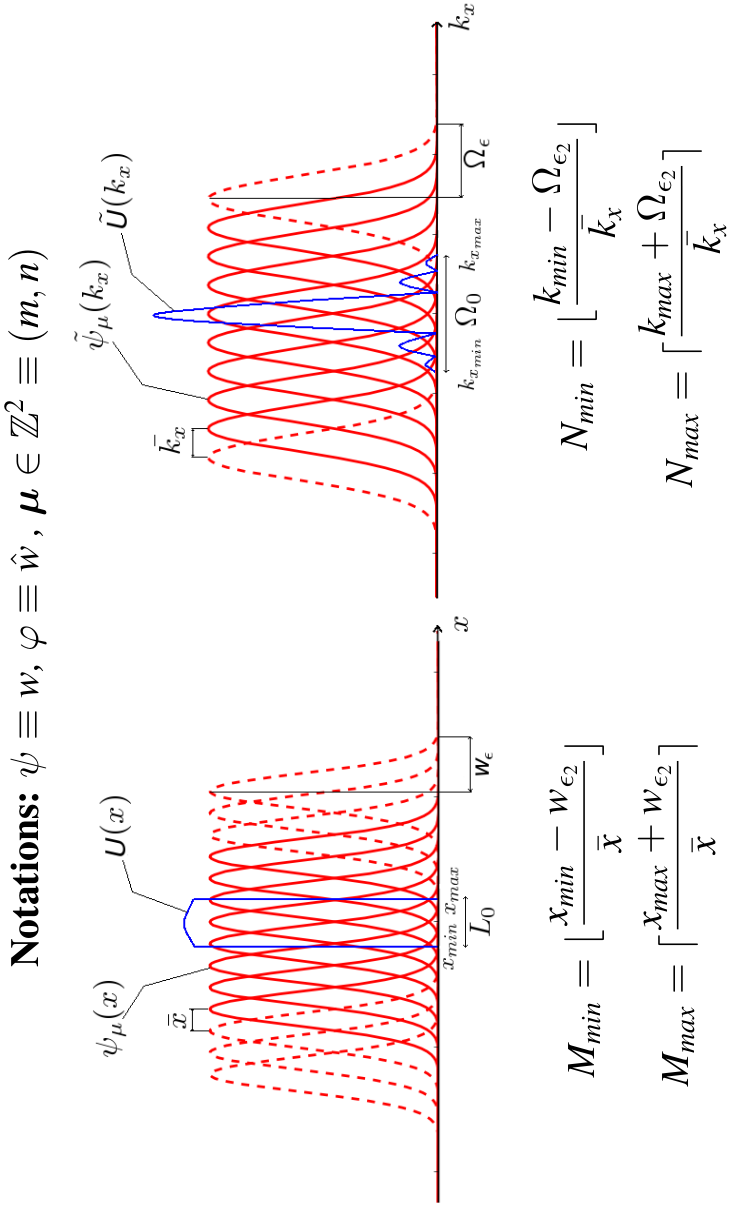
\includegraphics[scale=0.8]{minmax.png}


\subsection{Calcul approché des fenêtres duales}


Dans la suite, nous présentons sur les mêmes figures les fonctions duales approximées à différents ordres
afin de valider la bonne reconstruction de ces fenêtres, avec selon les différentes valeurs de $\nu_x$,
principal paramètre agissant sur la convergence des fenêtres approximées vers la fonction duale.
\footnote{L'autre paramètre pertinent est $\b{x}$, mais dans notre travail,
celui-ci ne varie pas par hypothèse du frame équilibré (voir \eqref{Lx}).}
Dans les légendes des figures suivantes,
les notations de variables se veulent \og phonétiquement cohérentes\fg\ avec ce rapport.
Précisons que $\eepsilon$ et $N_x$ désignent le seuil de précision
et le nombre de points utilisés pour calculer $\h{\t{w}}$.


\subsubsection{$\nu_x = 0.25$}


\paragraph{}

Comme annoncé dans \cite{TheseLugara}, c'est le cas pour lequel la convergence de l'algorithme est la plus rapide.

Les ordres $1$ et $2$ d'approximations sont quasi-indistinctibles, et selon la précision souhaitée (ici $10^{-3}$),
l'approximation à l'ordre $0$ peut-même être acceptable: $\h{\t{w}}\simeq\alpha_{00}^0\t{w}=\f[1]{\pi(A_x+B_x)}\t{w}$

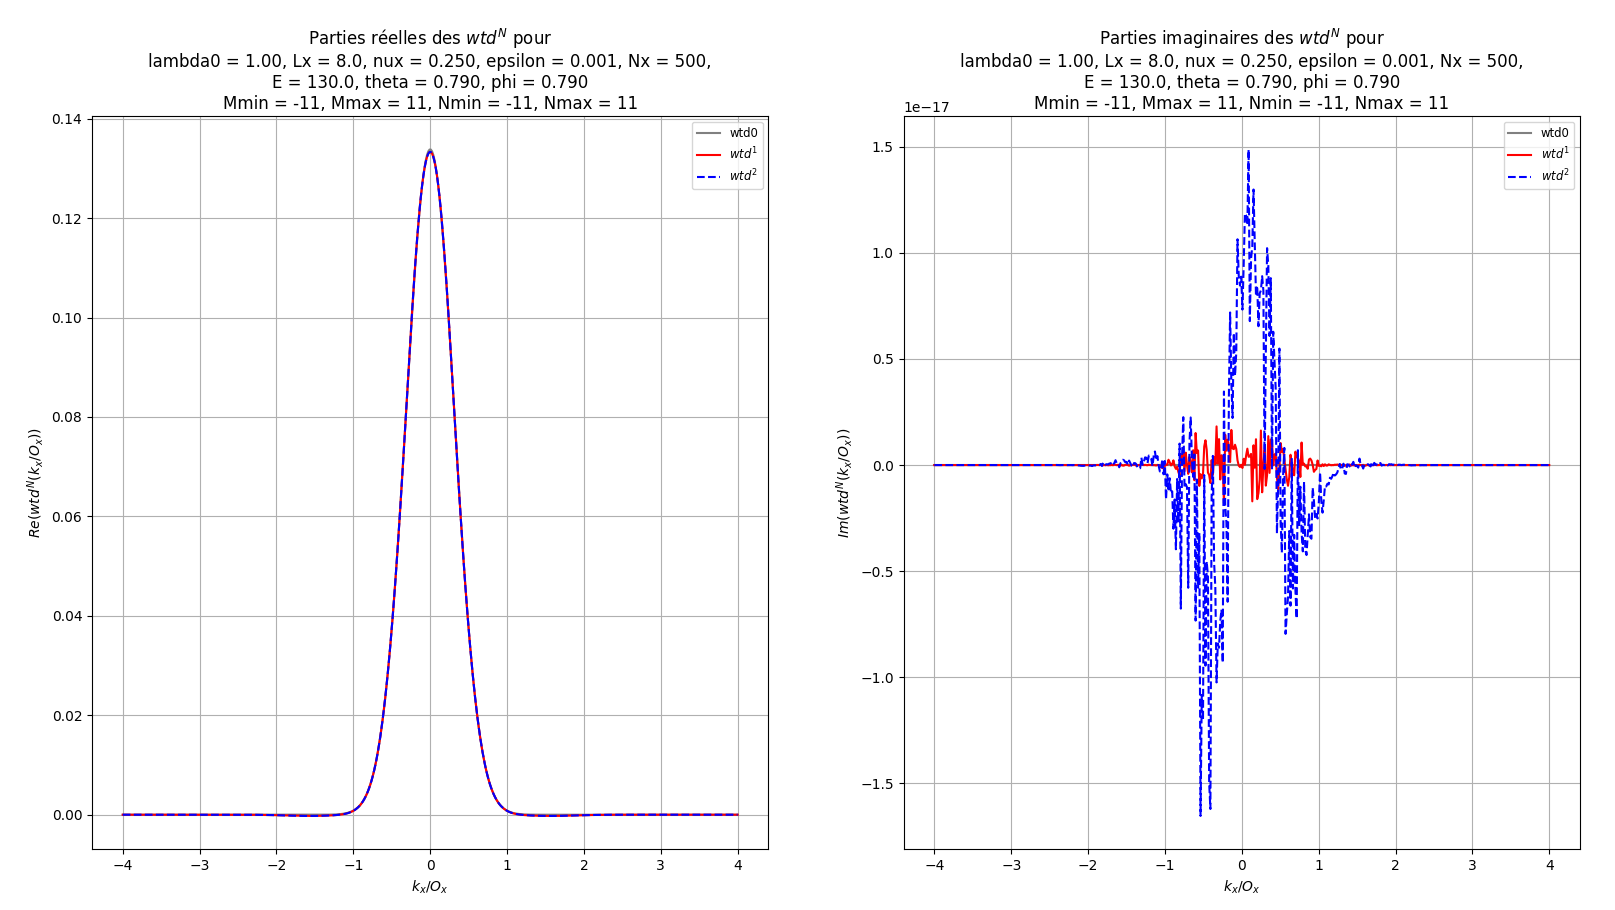
\includegraphics[scale=0.35]{1.png}

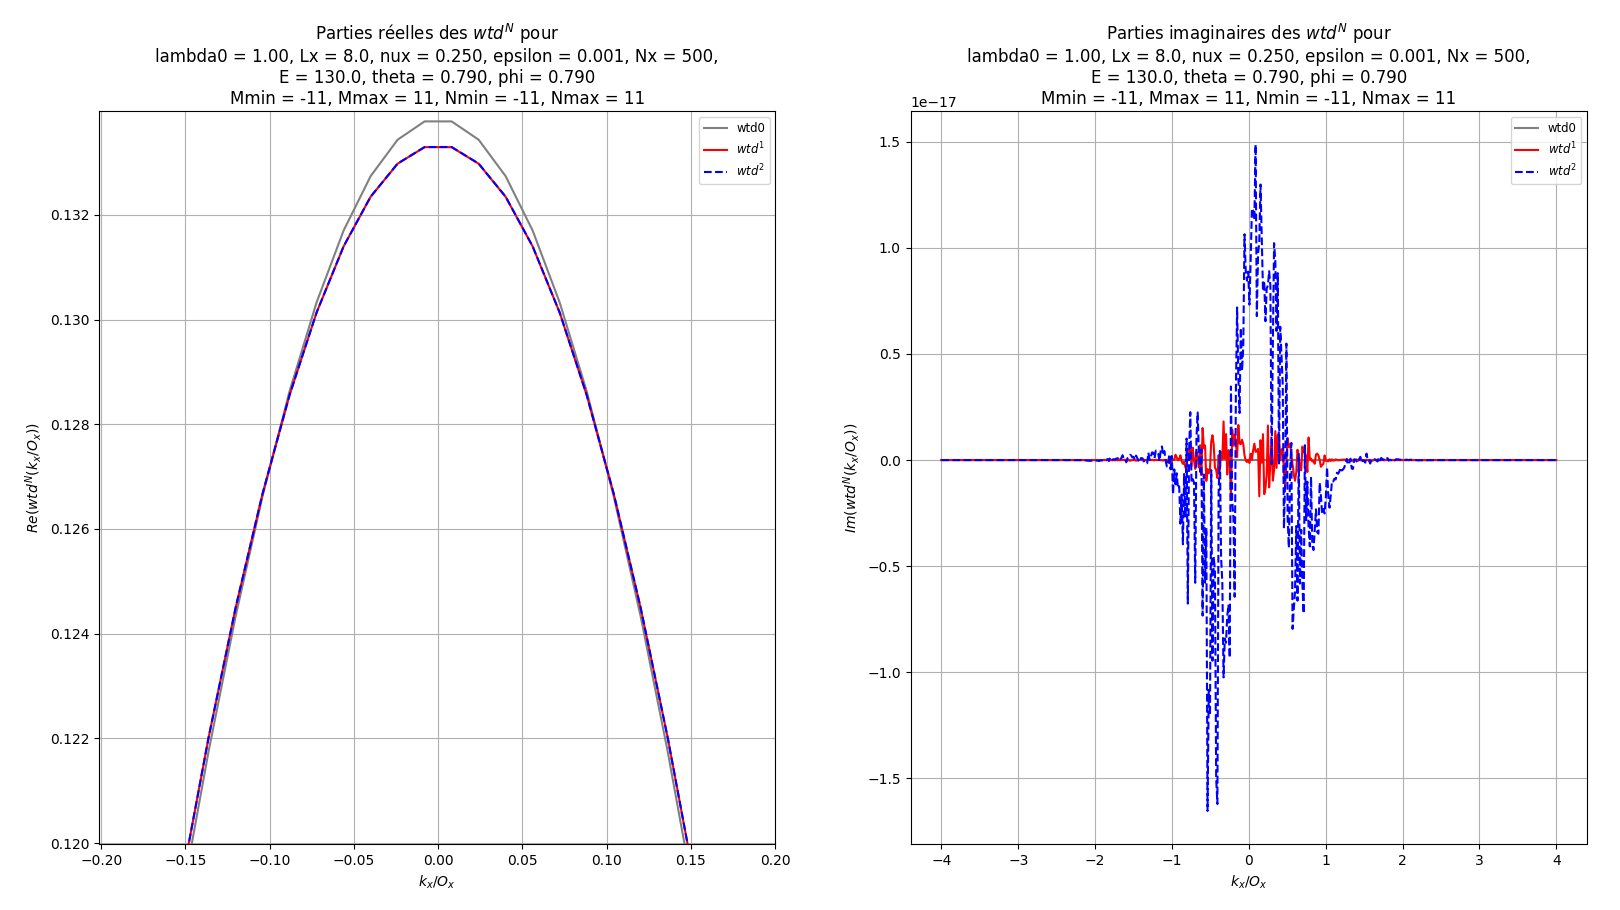
\includegraphics[scale=0.35]{1-1.png}

\newpage

Concernant la partie imaginaire de $\h{\t{w}}$ ainsi approchée, il se trouve qu'elle est d'amplitude extrêmement faible
(de l'ordre de $10^{-17}$, ce qui est négligeable devant le seuil de précision choisi). Son irrégularité peut faire
d'abord penser à des valeurs nulles, avec une erreur due à la résolution finie des faibles valeurs décimales
que l'ordinateur garde en mémoire,
mais il est possible d'atteindre une précision bien supérieure, même avec le language Python,
qui a été utilisé ici en raison de mes connaissances limitées en C++.
On constate donc (pour toutes les valeurs de $\nu_x$) que les parties imaginaires des $\h{\t{w}}^N$ sont négligeables
mais non nulles, ce qui est cohérent avec \eqref{alphanmN} (définie avec le terme comportant l'exponentielle).
\footnote{Les figures pour les autres valeurs de $\nu_x$ etant donc similaires,
elles n'ont pas été commentées dans la suite.}


\subsubsection{$\nu_x = 0.375$}

Pour cette faible valeur de $\nu_x$, la ressemblance entre les $\h{\t{w}}^N$, et la gaussienne initiale $\t{w}$
est encore correcte.
On commence certes à constater que l'ordre d'approximation nécessaire pour une bonne reconstruction de $\h{\t{w}}$
augmente avec la valeur de $\nu_x$, mais à ce seuil de précision, les faibles ordres $1$ et $2$ restent proches
et satisfaisants.

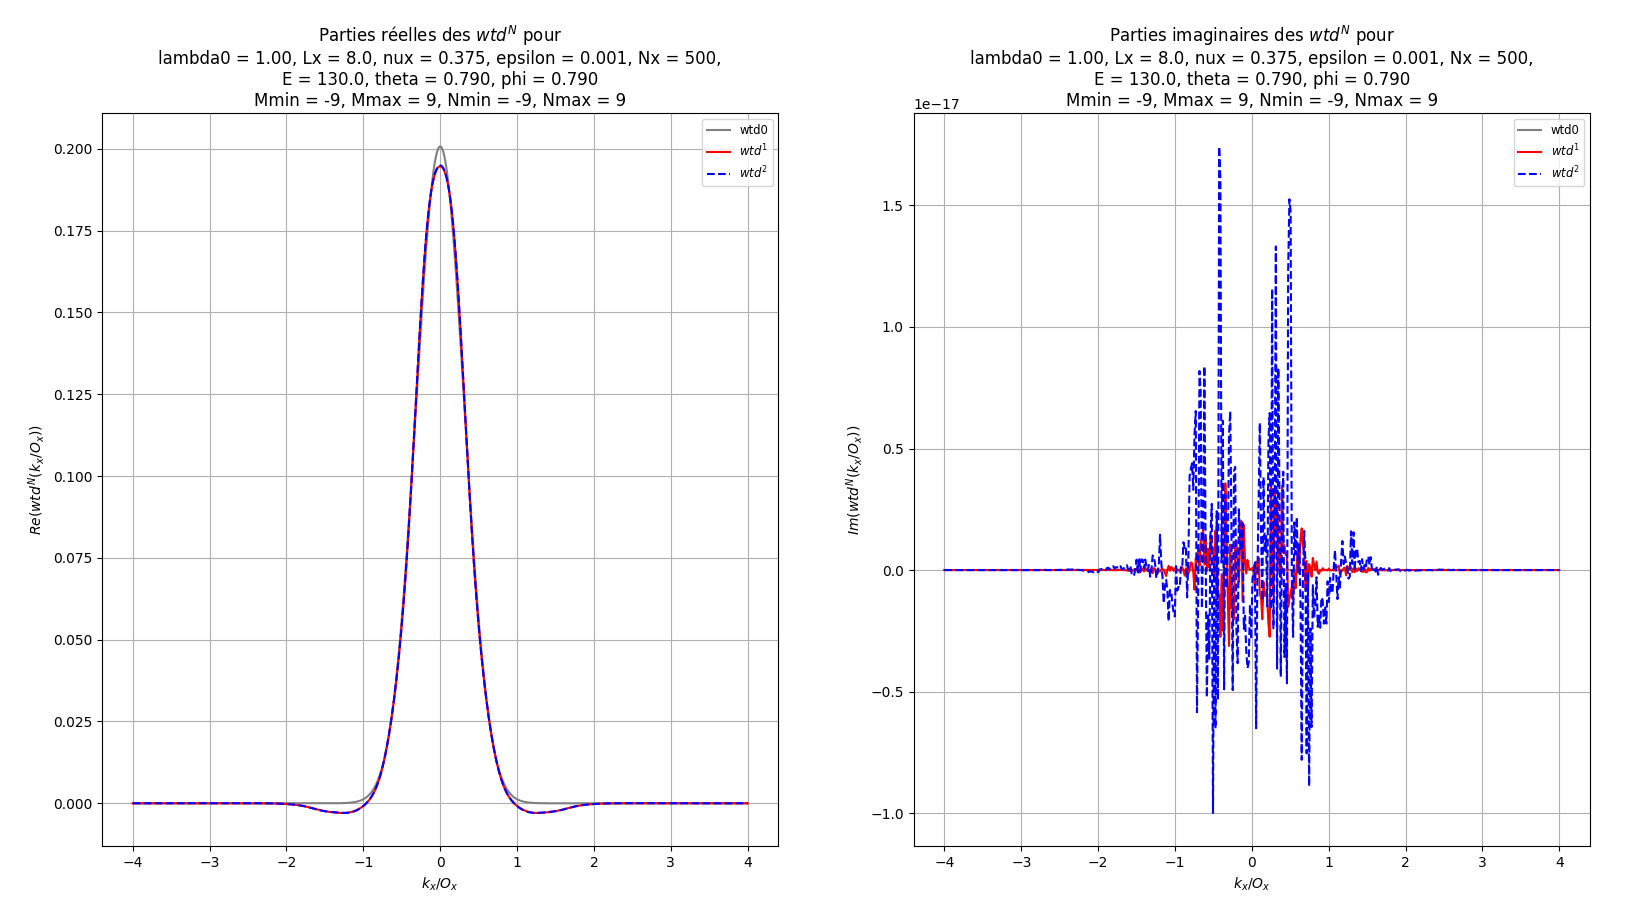
\includegraphics[scale=0.35]{2.png}

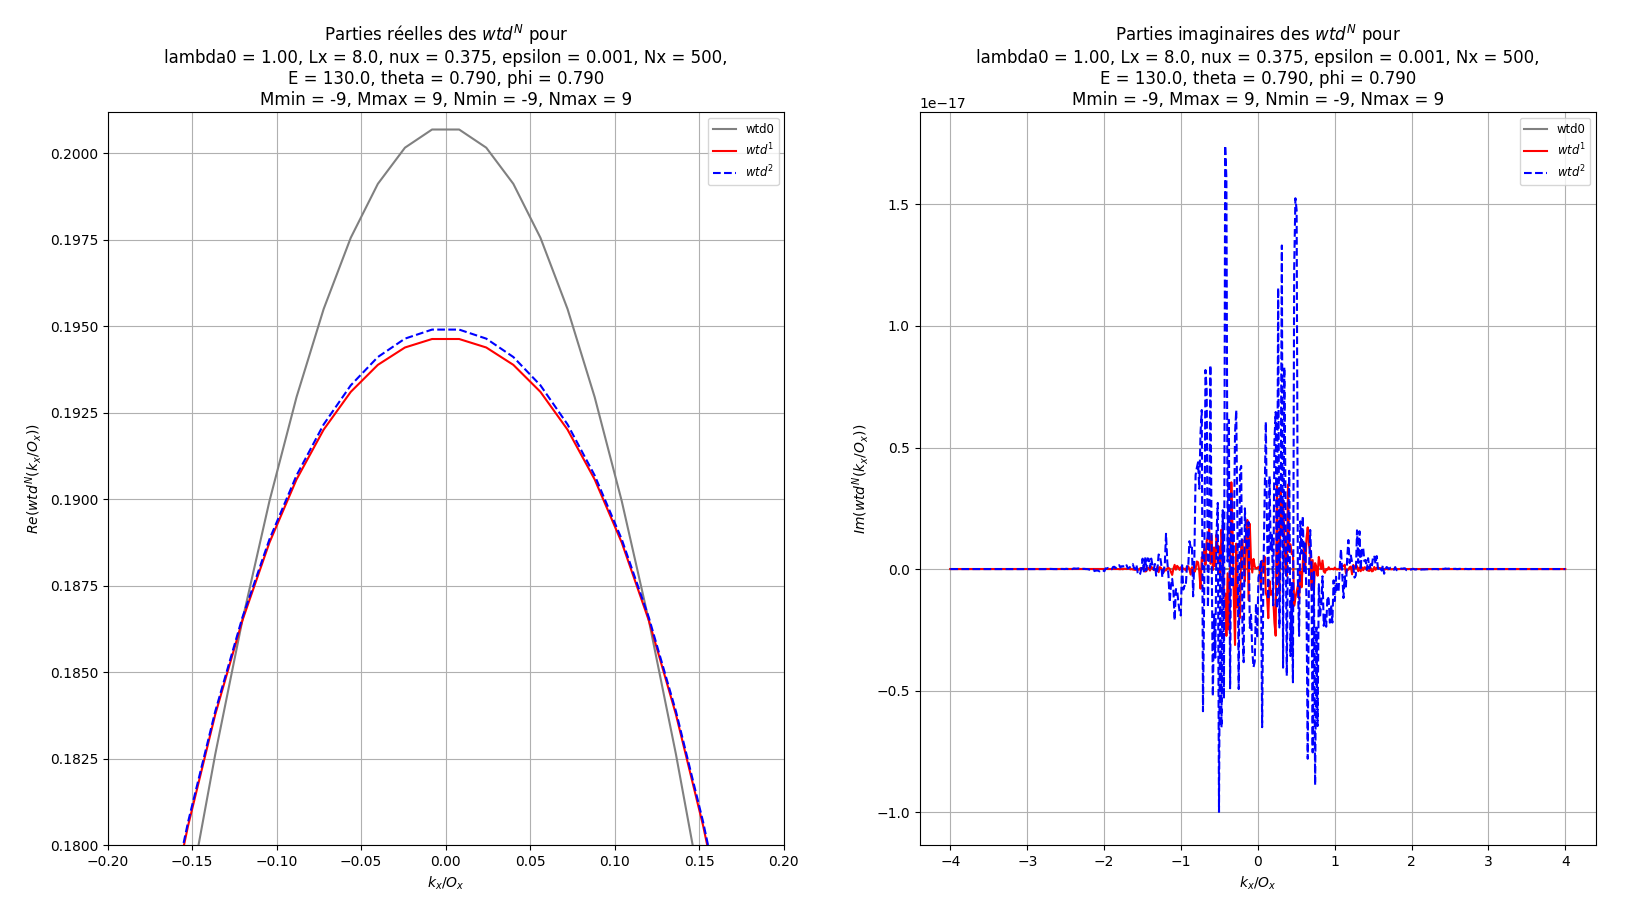
\includegraphics[scale=0.35]{2-1.png}

\newpage

\subsubsection{$\nu_x = 0.5$}

À partir de $\nu_x = 0.5$, les $\h{\t{w}}^N$ commencent à avoir une forme différant vraiment de $\t{w}$.


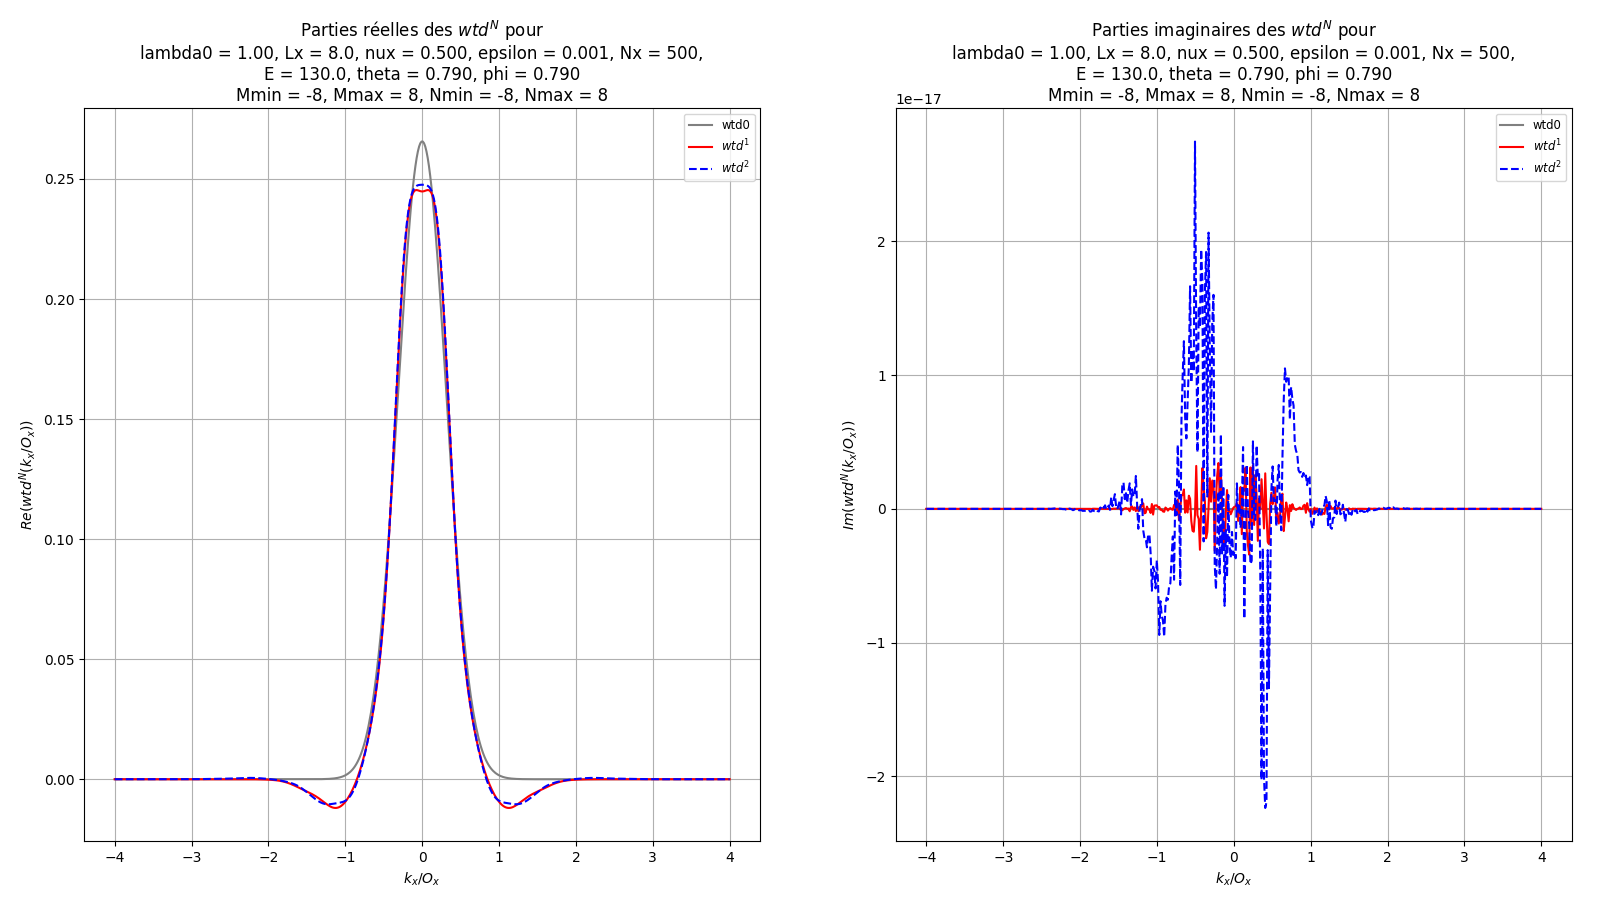
\includegraphics[scale=0.4]{3.png}

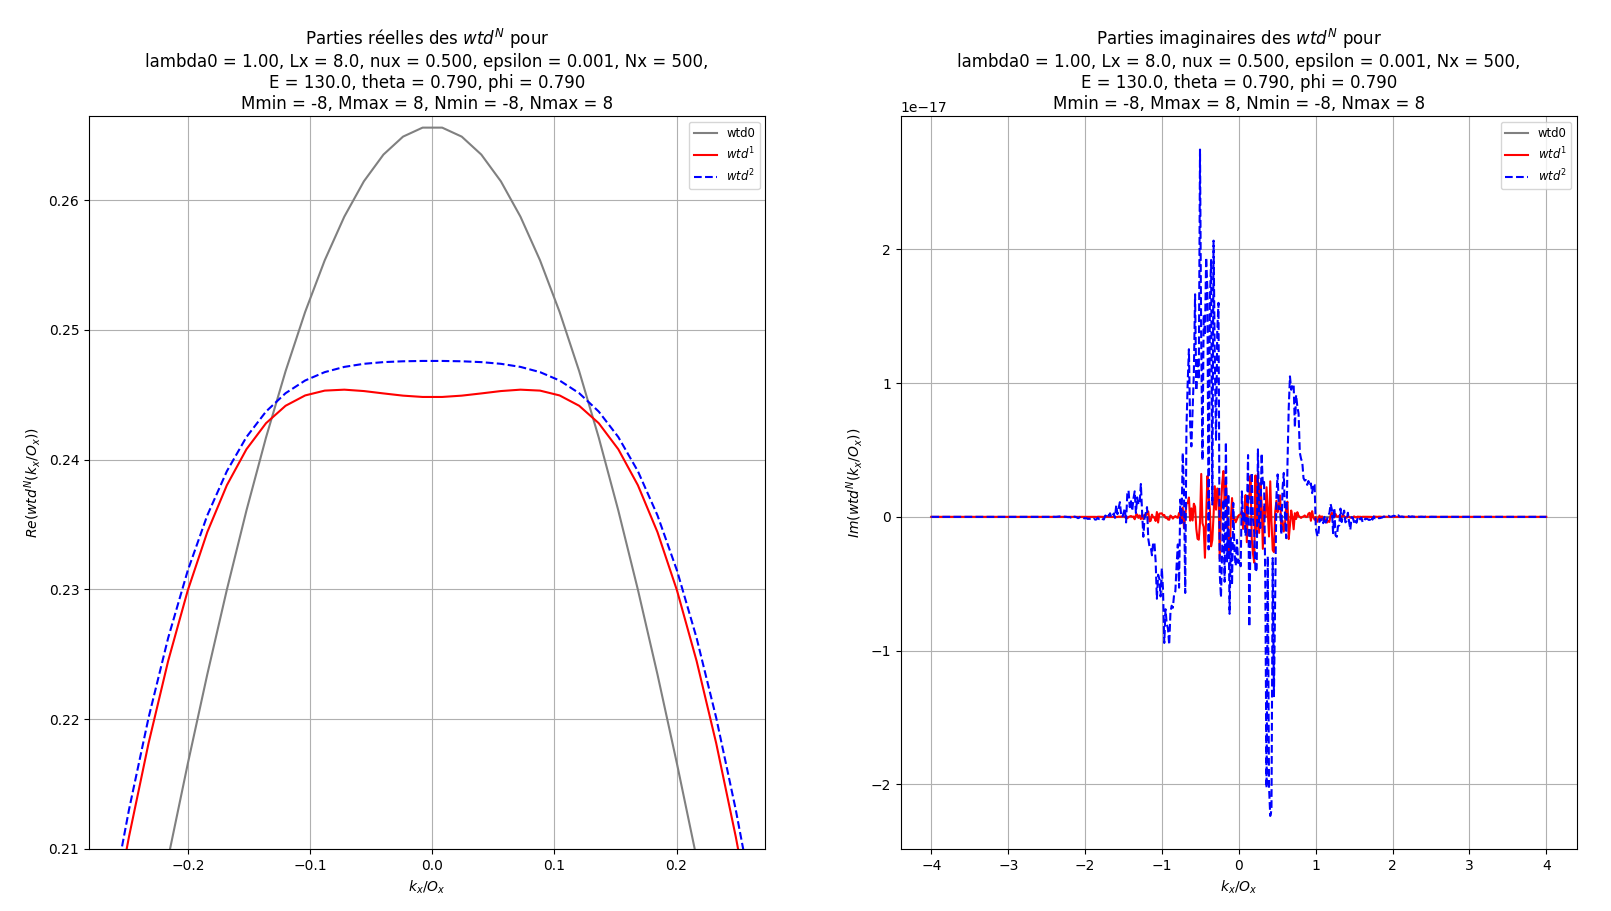
\includegraphics[scale=0.4]{3-1.png}


Ce constat, avec la plus grande différences entre les ordres $1$ et $2$ d'approximations, nous poussent donc à délaisser
les valeurs de $\nu_x$ supérieures à $0.25$ ou $0.375$ pour la reconstruction de l'onde globale.
\footnote{Les résultats trouvés au 22 juin 2017 ont d'ailleurs été trouvés avec
$\nu_x=0.25$, pour des raisons de délais et de performances.}

\newpage

\subsubsection{$\nu_x = 0.75$}

Comme déjà su, lorsque $\nu_x$ se rapproche de 1, les fonctions duales se rapprochent de la fonction biorthogonale
de la décomposition de Gabor (quand $\nu_x=1$, à ne pas confondre avec la décomposition sur un frame de Gabor en général).

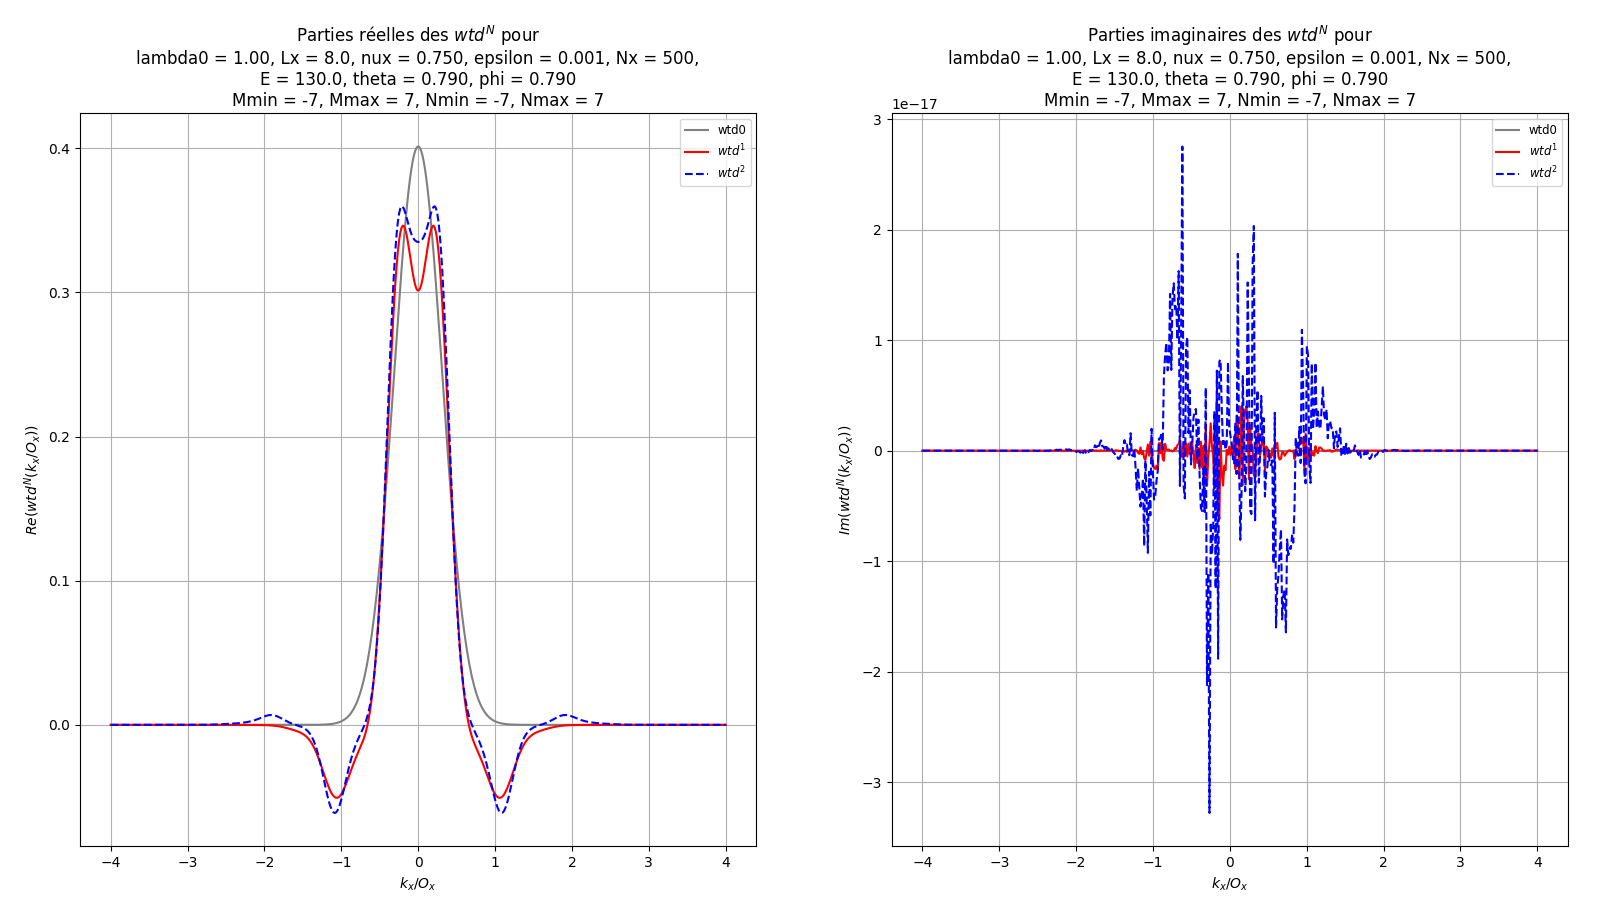
\includegraphics[scale=0.4]{4.png}

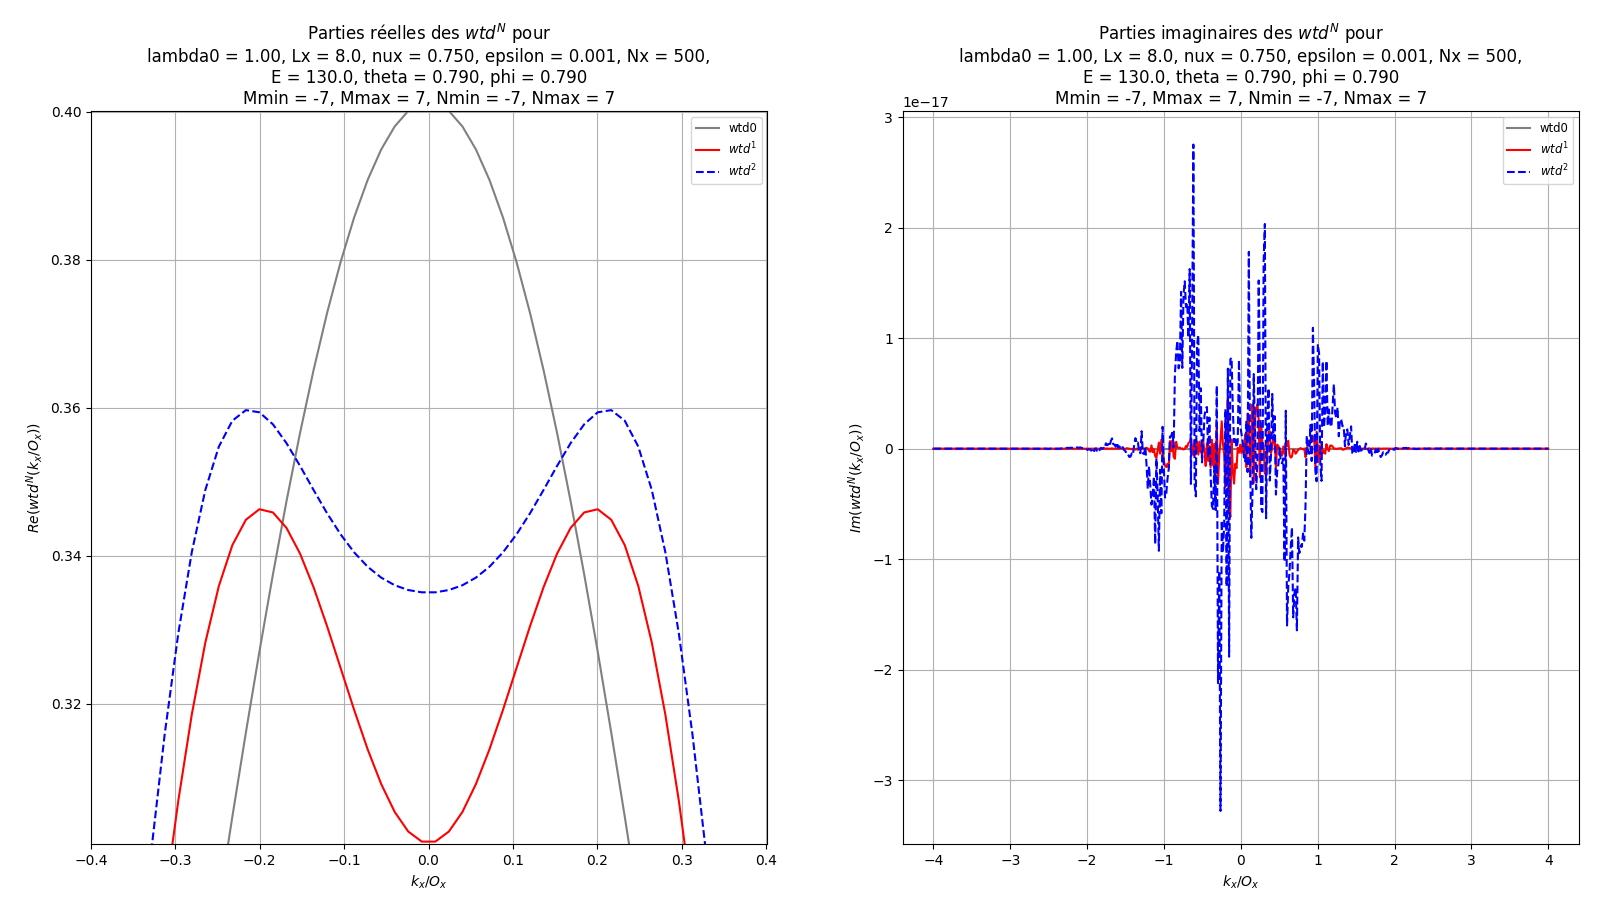
\includegraphics[scale=0.4]{4-1.png}


\subparagraph{}

En conséquence de ces résultats, nous faisons donc le choix de tenter la reconstruction de $\v{E}$ avec $\nu_x=0.25$,
car c'est la valeur nous donnant le plus rapidement, à l'ordre le plus faible (dès l'ordre $0$ voire l'ordre $1$),
la reconstruction la plus correcte de $\h{\t{w}}$.

%\newpage